\section{Introduction}

\paragraph{Research Question:}
\begin{quote}
    To what extent can a player travel in distance/displacement through a jump action in optimistic conditions of vanilla settings, within the games made with the source engine?
\end{quote}

The problem originated from my personal curiosity within the limitations of the video game ``Counter Strike'' that occupies a large part of my life. It came about as I was getting into the community of counter-strike long jumping --- a community aiming to exploit the video game's physics to achieve the longest jumping distance. Therefore I want to explore this optimization problem with various methods in an extended essay to further improve my knowledge within this ``niche`` community.

\subsection{Defining the problem}
The ``source'' game engine (citation) is the engine of plenty of popular videos games in terms of handling the players, their surroundings, and their respective physical interactions. It allows freedom in setting various engine constants that fit each video game's playstyle --- with the constants of ``Counter Strike - Source`` being used as a reference throughout this exploration. I will attempt to define the problem mathematically in this section.

% from p0 to p1, and to finishing this essay
Firstly, here is a run down of all the notations used in this analysis:

All n-dimensional vectors are represented in bold styles like
\[
\tvec{v},
\]
their magnitudes, or length are denoted by two double vertical lines, with the components of a vector written as a subscript $x$, $y$, or $z$ like
\[
\tmag{\tvec{v}} = \sqrt{v_x^2 + v_y^2 + v_z^2}.
\]

The vector can also be expanded into its components, and is written with angled brackets or with square brackets:
\[
\tvec{v} = \tang{v_x, v_y, v_z} = \tpars{v_x}{v_y}{v_z}.
\]

The unit vectors are vectors scaled down by their magnitudes, resulting in a magnitude of 1, and is written with a hat on top:
\[
\tunit{v} = \frac{\tvec{v}}{\tmag{v}}.
\]

The dot product between two vectors $\tvec{v}$ and $\tvec{w}$ is defined by
\[
\tvec{v} \cdot \tvec{w} = v_x w_x + v_y w_y + v_z w_z + \ldots.
\]

In addition, the absolute, floor, and ceiling piecewise functions are represented with
\[
    |x|, \floor*{x}, \ceil*{x}.
\]

Due to the nature of the source engine, the problem may be represented and optimized differently because of the use of discrete time frames rather than continuous time. But experimentally the differences are small and insignificant --- this will be shown later. Both approaches will thus be used, sometimes interchangeably.

The problem can be formally defined as so:
\begin{quote}
    Given initial position $\tvec{p}(0)$ and velocity $\tvec{v}(0)$ as three dimensional vectors when the player initializes a jump event, and a list of engine constants $S = \{j_0, j_1, j_2, \ldots\}$. If $\ta(t)$ is the acceleration vector function representing the player acceleration at every time $t$, with $\tv(t, S)$ and $\tp(t)$ being the respective derived velocity and position of the player at time $t$, what is the maximum displacement $\tmag{\tp(t_f) - \tp(0)}$ achievable if $t_f$ is the time when the player lands from the jump?
\end{quote}

\subsection{Source mechanics}
\label{sec:source}
While the problem may look simple in the context of kinematics and projectile motions, the ``quirks'' in the source engine will increase its complexity. Therefore it is necessary to explore the specifics of the physics engine.

The engine time unit is in seconds; the engine distance unit is in hammerunits (hu), which are to be implied for the rest of the analysis. The player's position and velocities are represented by 3-vectors $\tp$ and $\tv$ in the engine, which are updated every frame by the player controllable acceleration 2-vector $\ta$. Commonly, the source engine runs at an integer number of frames per second (citation), the number $64$ will be used from now. Let $\tau$ be the time between frames (also know as $\Delta t$) and it has a value of $\tau = \frac{1}{64} \approx 0.0156 \si{s}$. For every $\tau$ seconds after $t=0$, the velocity is updated in the following sequence (citations):
\begin{enumerate}
    \item Apply gravitational acceleration
    \item Apply friction onto velocity
    \item Calculate magnitude of movement acceleration
    \item Apply movement acceleration
\end{enumerate}

% took 45 frames, v0 = 284hu/s, 60fps
\paragraph{Step 1} Let $g$ be the gravitational acceleration on the $z$ axis, it is set by an engine constant \verb|sv_gravity| (citations) --- represented by variable $-g$ set to $800$ within the game in question. Using a method called leapfrog interpolation, and let $\tv'$, $\tp'$ be the new velocity, position next frame, the operation is (assuming $g$ is negative)
\begin{align}
    \tv'_z &= \tv_z + g\tau \label{eq:gv}\\
    \tp'_z &= \tp_z + \tv_z\tau + \frac{1}{2}g\tau^2 \label{eq:gp}.
\end{align}

Because the updates reflect the kinematic equations of a projectile with constant acceleration, it can be treated with assumption of continuous time and will be evaluated separately against the $x$ and $y$ motions.


\paragraph{Step 2} Let $\lambda(\tv)$ be the friction function. For the player is in the air, no friction will be applied and we can set $\lambda(\tv) = \tv$. After this section, the $\lambda$ function will be omitted as we are only considering air motions.

\paragraph{Step 3} The source engine limits the player velocity through an engine constant \verb|sv_maxspeed| ($L$) set to $30$ in air. However, the speed is limited by the projection of the velocity vector $\tv$ onto the acceleration vector $\ta$, with the player having control of $\ta$ at all times (figure \ref{fig:speedlimit}).

\begin{wrapfigure}{r}{0.45\textwidth}
    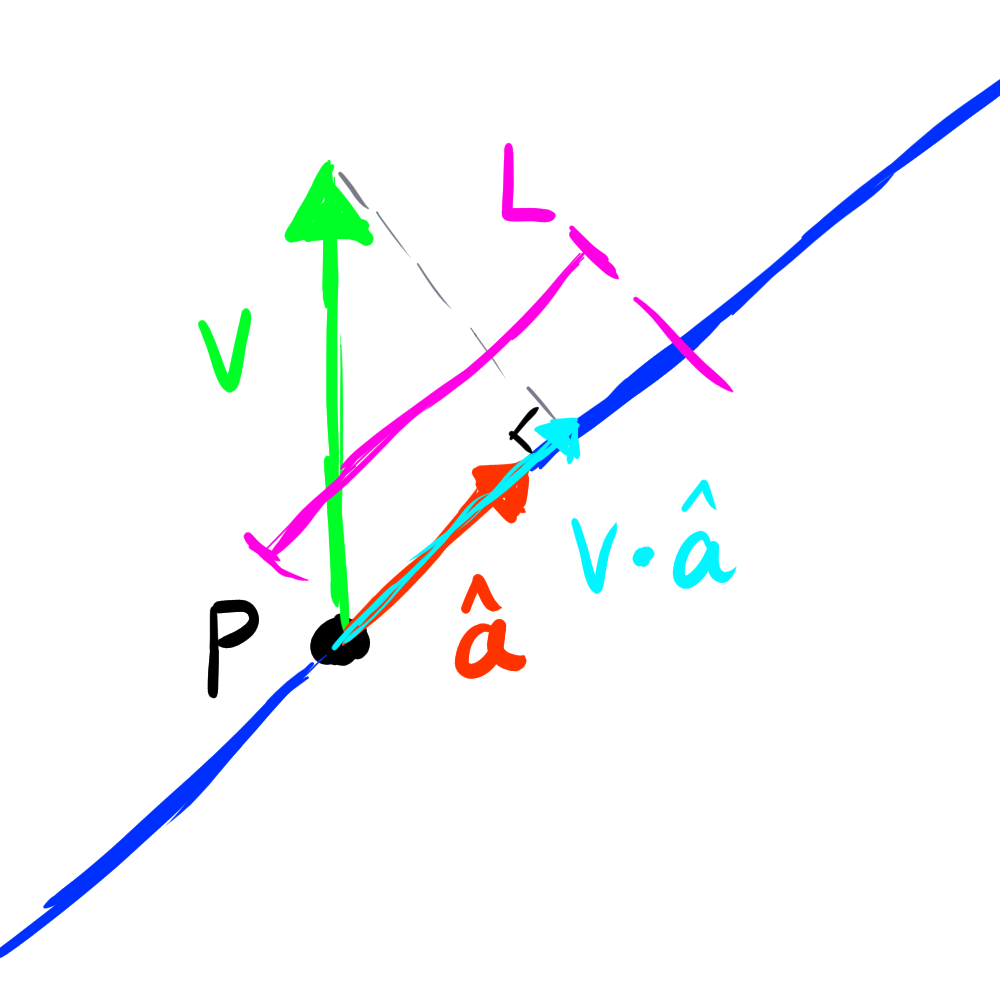
\includegraphics[width=0.43\textwidth,right]{assets/speedlimit.png}
    \caption{The speed limit}
    \label{fig:speedlimit}
\end{wrapfigure}

Let $w$ be the magnitude of the applicable acceleration this frame. It can be defined as a piecewise function as
\[
w = \begin{cases}
    \gamma_1 & \gamma_2 \ge \gamma_1\\
    \gamma_2 & \gamma_1 > \gamma_2 > 0\\
    0 & 0 \ge \gamma_2,
\end{cases}
\]
where the definition of $\gamma_1$ and $\gamma_2$ are:
\begin{align*}
    \gamma_1 &= LA\tau\\
    \gamma_2 &= L - \tv \cdot \tunit{\ta},
\end{align*}
where the dot product $\tv \cdot \tunit{\ta}$ with the unit acceleration vector represents the projection of velocity onto the acceleration vector.

The variable $\gamma_1$ is a constant represents the highest acceleration and is proportional to the engine constant \verb|sv_airacclerate| ($A$), and \verb|sv_maxspeed| ($L$); variable $\gamma_2$ is a function of $\tv$ representing the signed the difference between $L$ and the projected velocity.

When $\gamma_2$ is negative, meaning the projected velocity is larger than the max speed, no acceleration will occur and $w=0$; when $\gamma_2$ is positive but below $\gamma_1$, meaning that adding the full acceleration will overshoot the max speed, only the difference between the max speed and the current projected velocity is applied, bringing the player to the speed limit on the next frame and $w=\gamma_2$; when $\gamma_2$ is larger than $\gamma_1$, only the upper-bound acceleration is applied and $w=\gamma_1$.



\paragraph{Step 4} The new velocity on the next frame $\tv'$ (note that we assume step 1 has already been applied this frame) is the combination between the friction and movement acceleration:
\begin{align}
    \tv' &= \lambda(\tv) + w \tunit{\ta}\label{eq:dis_vel},
\end{align}
with the position being updated without interpolation ($\tp'$):
\[
\tp' = \tp + \tv' \tau.
\]

% jumping mechanics
% took 45 frames, v0 = 284hu/s, 60fps
Additionally, the mechanics of initiating a jump action can also be modelled mathematically. By recording myself jumping ingame at 60 frames per second (picture), I've obtained that a jump is represented by an impulse applied on the player, setting its z-axis velocity $v_{0z}$ to around $+280\pm10$ the frame after jumping. The player then takes around $45 \pm1$ video frames to land, meaning an airtime of $45 / 60 =0.75\pm 0.02\si{s}$. Therefore the initial velocity is restricted by $\tv_z = 280\pm10$.

% summarize
To summarize, every $\tau$ seconds after $t=0$ the velocity is updated by gravity in the z-axis, and by the player's movement acceleration in the x,y-axis. The latter is limited so that the projection of the new velocity never exceeds the engine constant \verb|sv_maxspeed| of 30 in air. Therefore for some time $t$, the velocity next frame $\tv(t+\tau)$ is
\begin{align*}
    \tv(t+\tau) &= \tang{\tv_x(t) + w \tunit{a}_x, \tv_y(t) + w\tunit{a}_y,\tv_z(t) + g\tau}\\
    \tp(t+\tau) &= \tang{\tp_x(t) + \tv(t+\tau)_x \tau, \tp_y(t) + \tv(t+\tau)_y \tau, \tp_z(t) + \tv_z(t)\tau + \frac{1}{2}g\tau^2}.
\end{align*}
